\subsection {Session 5, Exercise 3}

\label{6_3}

\lineparagraph {Exercise}

The following table contains the transition function of a 2-tape Turing machine, where $*$ is the blank symbol on the tapes, and $q_0$ is the start state.

\begin{center}
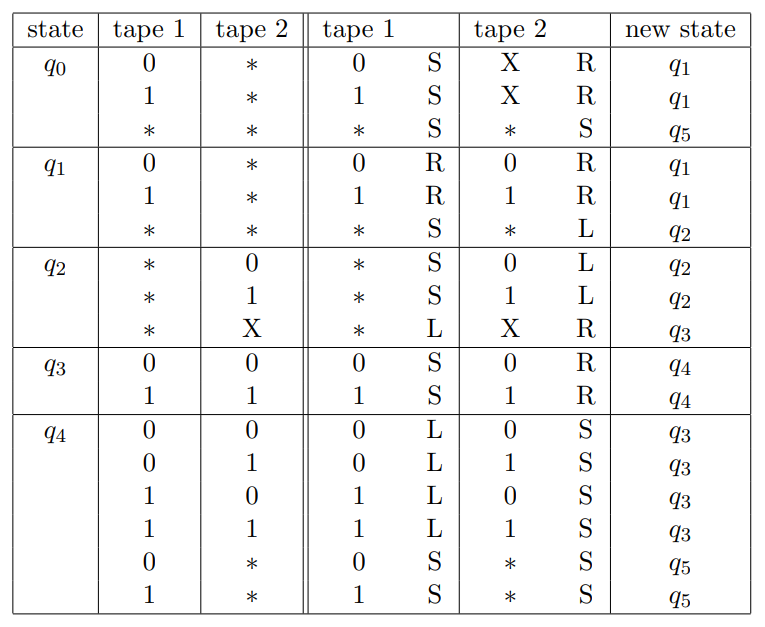
\includegraphics[width=0.7\linewidth]{05/6_3_task.png}
\end{center}

\begin{enumerate}[a)]
    \item What is the content of tape 2 when the machine moves to state $q_2$?
    \item What is the language $L(M)$ if the only accept state is $q_5$?
    \item At most how many steps are done by the machine on an input of length $n$ before it stops?
\end{enumerate}

\lineparagraph {Solution}

To see a little bit easier what this TM does, I converted it line-by-line to the below form:

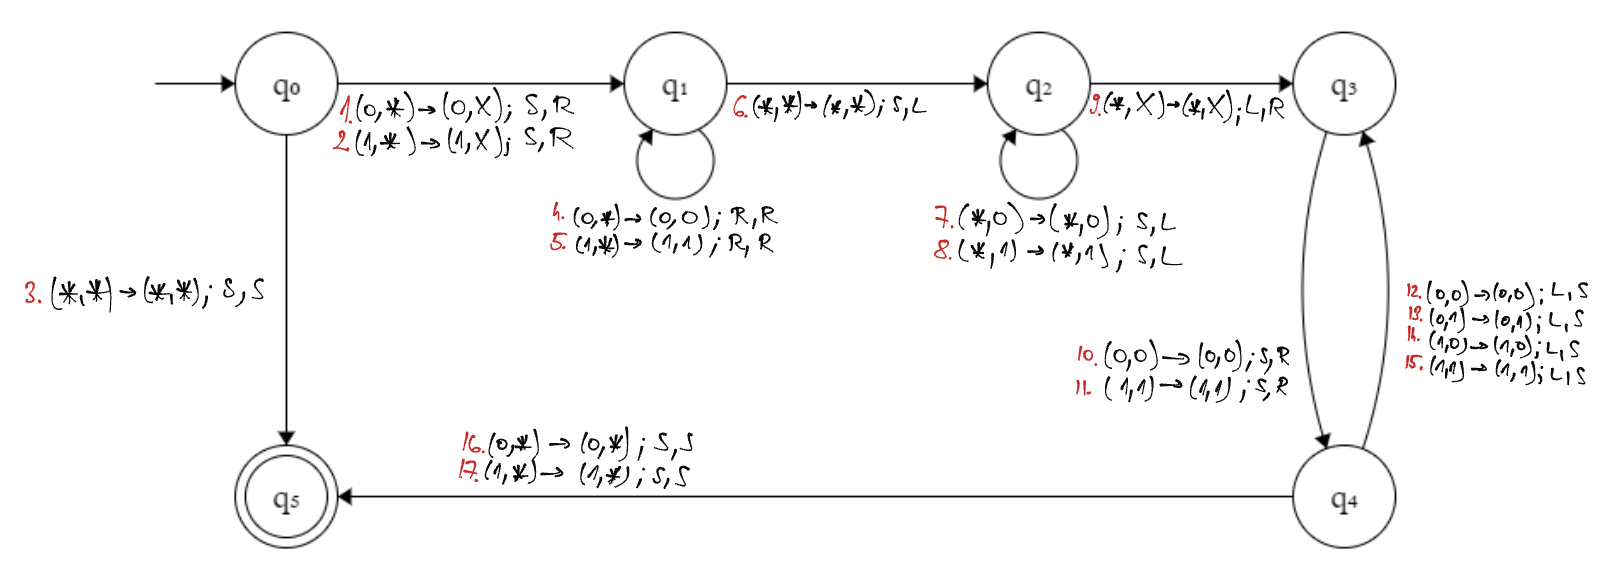
\includegraphics[width=\linewidth]{05/6_3_canvas.png}

What this does:
\begin{itemize}
    \item Transition 3: This one handles the empty string input and immediately moves to the accept state $q_5$. So the empty string is accepted. So the empty string is accepted in $1$ step. For any other input, the following happens:
    \item Transitions 1-2: They put down an $X$ character at the beginning of the second tape. This $X$ will be used later to make sure that the head does not fall of the tape (moving from the first position to the left would cause the head to fall off, this $X$ is there so we can detect it and make sure no transition is defined that moves the 2nd head to the left when it reads an $X$). This is $1$ step.
    \item Transitions 4-5: They copy the first tape's contents to the second tape. This is $n$ steps if the input is of length $n$.
    \item Transition 6: When the on the first tape the head is at the end of the input word (sees the $* =$ empty cell character we move to state $q_2$ and we position the second head on the last character of the copied input. (While the first head remains on the $* =$ empty cell after the input.) This is $1$ step.
\end{itemize}

a) When we move to state $q_2$ the contents of tape $2$ will be the character $X$ at the beginning, then the input word copied afterwards.

\begin{itemize}
    \item Transitions 7-8: The first head stays on the same $*$ cell, while the second had moves to the left until it finds the character $X$ (beginning of the second tape). This is $n$ steps if the input is of length $n$.
    \item Transition 9: The first head is positioned at the end of the input word, while the second head is positioned at the beginning of the (copied) input word. This is $1$ step.
    \item Transitions 10-15: Together these make $2n$ steps for an input word of length $n$, see explanation below:
    \begin{itemize}
        \item Transitions 10-11: These compare the two strings (the input word twice, on the first tape from right to left and on the second tape from left to right). However, the first head is not moved immediately to the left. This is because the first head could fall off the first tape, since there is no protective $X$ there. We cannot recklessly move to the left.
        \item Transitions 12-15: Instead we lag behind the second head and make sure that the second head reads either a $0$ or a $1$ (and the first head can read $0$ or $1$ as well), which means that the word has not yet ended! (The second head would read $*$ here when the word ends.) This means that it is \textbf{safe} to move the first head to the left, since it is not yet at the beginning of the tape, so we move.
    \end{itemize}
    \item Transitions 16-17: Finally, when the second head reads the empty cell, it means that the word has ended (and has been successfully compared), so we can move to $q_5$. We make sure that we \textbf{DO NOT} move the first head to the left in this step, since it would fall off. Since the first head could be on a character $0$ or a $1$ we need to define 2 transitions to cover all possibilities. We move to $q_5$ here. This is $1$ step.
\end{itemize}

Together the number of steps for a successfull computation has been (for a non-empty input):

\begin{itemize}
    \item Transitions 1-2: $1$ step.
    \item Transitions 4-5: $n$ steps.
    \item Transition 6: $1$ step.
    \item Transitions 7-8: $n$ steps.
    \item Transition 9: $1$ step.
    \item Transitions 10-15: $2n$ steps.
    \item Transitions 16-17: $1$ step.
\end{itemize}

At most $4n+4$, but keep in mind that for a rejecting computation the number of steps is smaller, depending on where it halts in transitions 10-15. (At least $2n+3$ steps, since copying and moving the second head back to the first position will be done regardless of rejecting / accepting.)